%3.3
\section{アルゴリズムの構築}\label{chap:3.3}
この節では,排泄検知に関する関連製品とそれらのアルゴリズムの概要ならびに本研究におけるアルゴリズム構築および検証とその結果について述べる.

\subsection{排泄検知に関する関連製品とアルゴリズムの概要}\label{chap:3.3.1}
まず,他の排泄検知に関する関連製品がどのような方法を用いて検知しているか述べる.排泄検知をする際の方法としては,以下の3通りが挙げられる.

\begin{enumerate}
\item ガスセンサ方式を用いた排泄検知
\item 濡れセンサ方式を用いた排泄検知
\item その他のセンサ方式を用いた排泄検知
\end{enumerate}

一つ目のガスセンサを用いた製品に関しては2.4節に既に述べているため割愛する.二つ目の濡れセンサを用いた製品では,竹中エンジニアリング株式会社により2000年に発売された「おむつセンサキット」(?)や株式会社秋田テクノデザインにより2010年に発売された「おしりカイテキ」(?)などがあげられる.三つ目のその他のセンサを用いた排泄検知では,株式会社エヌウィックにより2012年に発売された「マインレット」(?)や有限会社アキテックにより2013年に発売された静電容量方式による「おむつセンサ『さわやか』」(?)などがあげられる.また,ユリケア株式会社により2004年に発売された「ゆりりん」(?)やTriple W Japanにより2017年に発売された「DFree」(?)は,超音波方式を用いているものの排泄検知ではなく,排尿予測を売りにした製品である.

★
\begin{figure}[htbp]
   \centering
   
\includegraphics[width=5cm]{./fig/temp.eps}
   \caption{類似製品分析 \cite{mic17a} }
   \label{mic17a}
\end{figure}

後述する本研究のアルゴリズムも紹介したシステムと同様に,排泄部周辺の空気を吸引することでガスセンサによる排泄検知を実現しているが,ガスセンサ値にはセンサ個体差や利用者の個人差によるばらつきが大きいため,それらを吸収するアルゴリズムを備えている点が異なる.

次に,排泄検知システムにおけるアルゴリズムについて述べる.\\
ここでのアルゴリズムとは,センサデータを用いて排泄検知を可能とするソフトウェア上の処理手順を指し示す.

先述した排泄検知に関連する製品は,そのハードウェア構造や使用方法によりアルゴリズムの処理概要を推測することが可能である.大きく分けて以下の2種類のグループに分類が可能であると考えた.

\begin{enumerate}
\item センサの出力値が2値(1と0,5Vと0V,など)となるものを用いて出力値の状態を基に判断する方法
\item センサが取得する物理量(空気中のガス濃度や温度,湿度など)が決められた一定の値(閾値)に達するか否かを判断する方法
\end{enumerate}

一つ目の方法では,接点スイッチや濡れセンサ(水などの液体による通電を接点とするもの)ような部品を使用していることが多く見受けられる.ハードウェアとしても単純な構造となり,アルゴリズムとしても「1」であるか「0」であるかという簡易な条件分岐のみで良いため複雑な処理の必要がない.例えば,ある製品ではおむつ内に濡れセンサを用いることによって排泄時を検知することが可能である.しかし,対象事象が特定の2値状態で分類可能であることやそれらの状態の境界を自由に決定できない.濡れセンサなどは,一度反応するとその状態を維持してしまうことなどもあるため,リセットや使い捨てによる交換など何らかの対応が必要である.前述の例では,濡れセンサが使い捨てとなっており,交換が必要である.\\
二つ目の方法では,利用するセンサの取得可能な値域内に任意で基準を設けることが可能であり,その基準値に従って条件分岐が可能であるため,設計者が任意の値を対象状態の境界に設定することが可能である.例えば,VOCなどに反応するガスセンサと温度センサを利用したある製品では,ある温度Tとセンサ値Cを処理し,放屁または排便(排尿)を検知することが可能である.しかし,利用するセンサの個体差やセンサ値を算出する際の分解能などハードウェアに依存してしまう部分や対象の状態が無数に存在することによるユニークな閾値決定の困難さなどが存在し,結果的にアルゴリズムの複雑化を起こし,処理時間の増加などの原因となる.前述の例では,設計者が決定したTやCの閾値が対象状態の実際の境界値ではない可能性があることが挙げられる.

★
\begin{figure}[htbp]
   \centering
   
\includegraphics[width=5cm]{./fig/temp.eps}
   \caption{閾値判定のアルゴリズム概念図}
   \label{mic17a}
\end{figure}

\subsection{本研究におけるアルゴリズム構築}\label{chap:3.3.2}
本研究におけるアルゴリズムは,実際の現場へ導入することを目的としていたため,一つのアルゴリズムで多人数に対応可能である必要があった.しかし,使用するTGS2602はセンサ自身に個体差を持っており,その差は比較的大きいものであった.較正(キャリブレーション)することも考慮したが,個人の排泄臭にも大きな差が生じる知見があったため,簡易的なものでは吸収が困難であると判断し,教師データを用いた機械学習に着目した.\\
初期の段階で健常者によるデータを用いた実験では,ある程度安定した波形かガスセンサから得られていたため,波形の局所的な特徴を用いていた.また,教師データとなる正解は常に記録されていたため,教師付き学習を用いることが容易であった.しかし,介護施設における実際のデータに関してはセンサ波形のバリエーションが多かったため,局所的な情報の使用を断念し,大局的な特徴量を用いることとした.さらに,実際の介護現場ではガスセンサの応答に対して正解を記録する作業が,非常に困難であることがわかり,教師付きデータの取得を断念した.本アルゴリズムでは,排泄データの部分時系列データをk-means法によって教師なしで排泄検知と排泄種類判別を行っている.

排泄検知アルゴリズムの概要フローチャートを\refFigJp{algo_flow}に示す.
\begin{figure}[t]
\centering
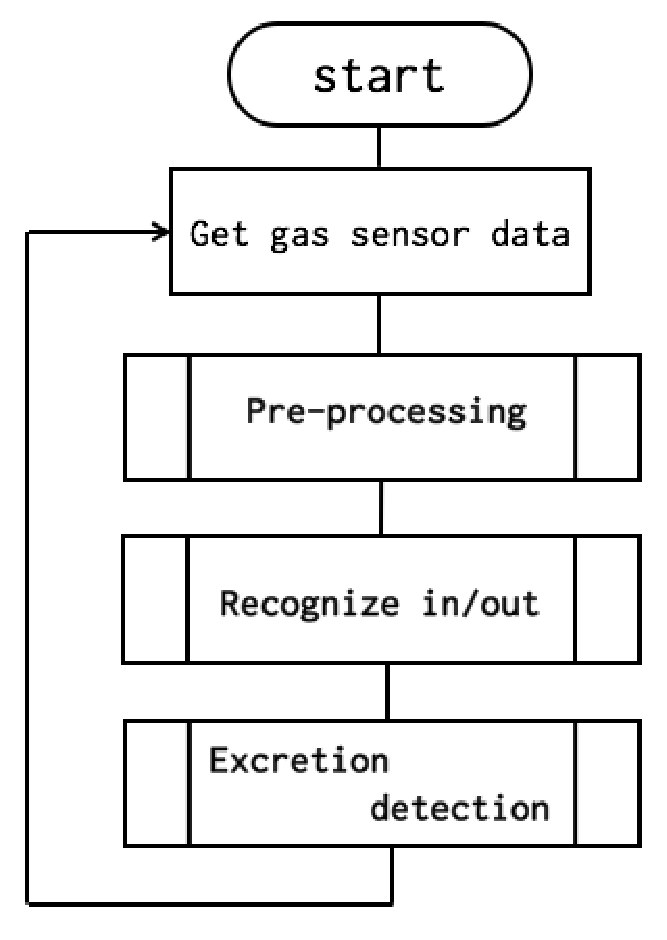
\includegraphics[width=5cm]{./fig/algoflow.eps}
\caption{アルゴリズムのフロー図}
\label{algo_flow}
\end{figure}

本研究で採用している排泄検知アルゴリズムは,大きく分けて以下の三つである.
\begin{enumerate}
\item 前処理部
\item 離着床判定部
\item 排泄検知部
\end{enumerate}

本研究では排泄検知部を二つ考え評価するものとする.ここで,その二つを排泄検知部I,I\hspace{-.1em}Iと名付けることとし,それらを採用した排泄検知アルゴリズムを排泄検知アルゴリズムIおよびI\hspace{-.1em}Iとする.すなわち,三つの処理のうち前処理部と離着床判定部は共通であり,排泄検知部のみが異なる.以下,詳しく説明する.

前処理部では,排泄データの移動平均をとり平滑化することを行う.\\
排泄によるガスセンサの応答は,立ち上がりを見せて再度落ち着くまで約1,2時間程度を要する制限が存在するため,瞬間的な波形の特徴パターンよりは比較的長時間の特徴パターンによって十分クラスタリングできると考えた.これまで知見から50秒の移動平均が最も適しているという結果を得ているが,区切りの良さと影響の程度を考慮した上で,1分の移動平均を取ることとした.\\
また,本アルゴリズムはこの移動平均値を15分単位の部分時系列データに分割された一つの窓として離着床,排泄検知に使用する.この窓のことを滑走窓と本研究では呼ぶ.\\

★
\begin{figure}[htbp]
   \centering
   
\includegraphics[width=5cm]{./fig/temp.eps}
   \caption{排泄検知アルゴリズムの特徴量概念図}
   \label{mic17a}
\end{figure}

離着床判定部では,利用者がベッド上に存在するかどうかを判定する.\\
過去において利用者が着床していない場合でも,ベッド付近の排泄臭以外に反応して通知してしまうことがあった.\\
そこで,離着床判定を取り入れることによって利用者が離床しているのにもかかわらず通知してしまう誤報を減らすことを目的とした.ここで正解率の高い離着床センサを併用することは,排泄検知をより正確にすることに貢献する.しかし,開発しているハードウェアは市販を目的としており,その利用に関してのコストを最小化することは大きな要求であった.その観点から,他の離床センサを使用することなく,現在使用しているセンサのみで離着床が判断できれば製品としての優位性が増すと考えた.よって,本研究ではガスセンサによる離床判定を取り入れた.
\begin{figure}[t]
\centering
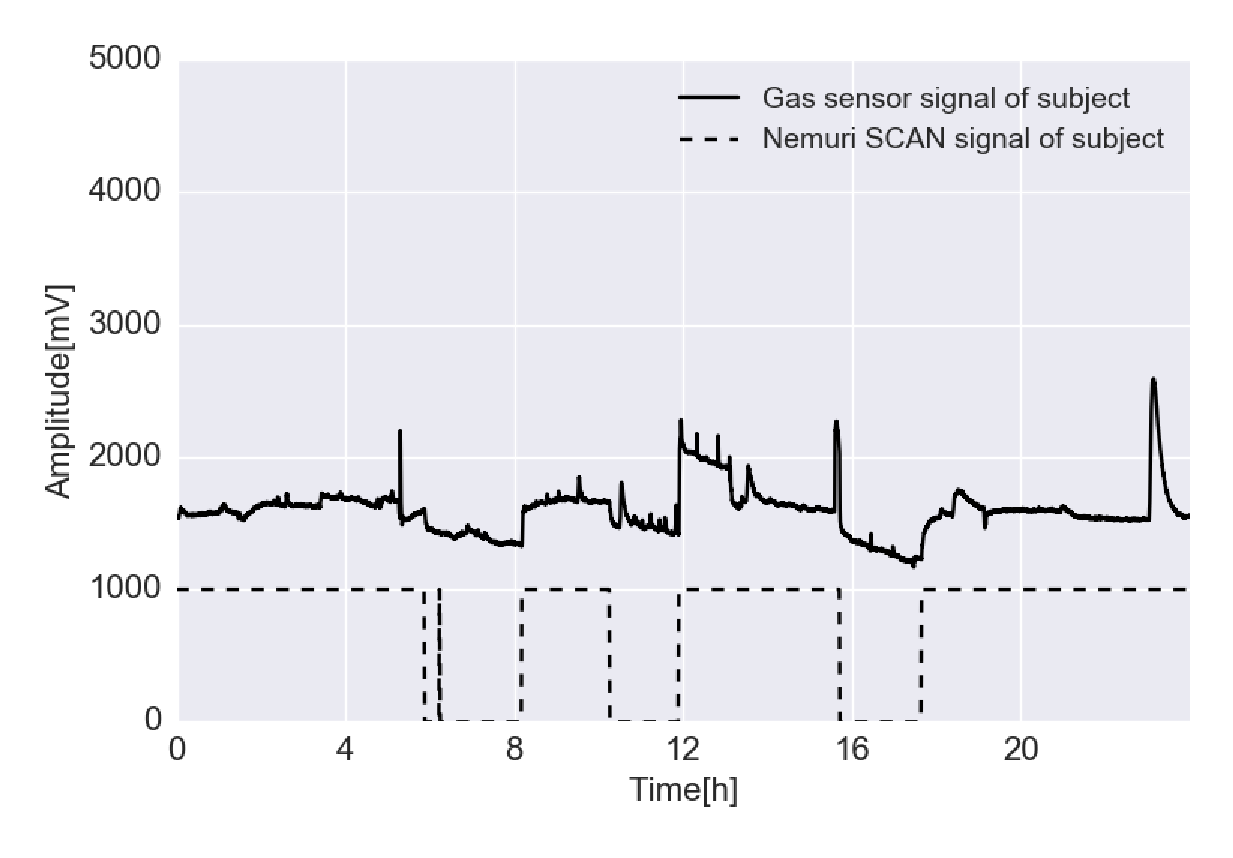
\includegraphics[width=8cm]{./fig/inout3.eps}
\caption{(JRMのFig.5)排泄センサーと睡眠センサー}
\label{inout3}
\end{figure}

\refFigJp{inout3}に移動平均によって平滑化した排泄データとパラマウントベッド株式会社の眠りSCANのデータを同時にプロットした例を示す.二つのデータは,それぞれのデータに記されているタイムスタンプをもとしている.ここで,眠りSCANはマットレスの下に敷くだけで睡眠状態の評価をすることができるデバイスである.眠りSCANは離着床データを出力することができるため,離着床判定部の評価に用いることができると考えた.\refFigJp{inout3}を見てわかるように,排泄データが離着床に応じて変化していることがわかったため,排泄データのベースラインを抽出することで,ガスセンサを用いて離着床判定を行うことができると考えた.\\

しかし,前述したようにTGS2602には個体差が存在し,個人の排泄臭や体臭の違いによる影響によって離着床時のベースライン値にばらつきが存在した.また,ベースラインを抽出できても排泄によるデータ変動により単純にベースラインだけで離着床を識別することは困難であった.そこで,被介護者の生活パターンに着目し,各時間帯における最頻値を統計的に抽出することで離着床判定をおこなうことを考えた.本研究では各時刻において頻出して測定されるガスセンサ値を最頻値と呼ぶ.\\
さらに,まるでスペクトログラムのように横軸を時間,縦軸にガスセンサ値,ヒストグラムの度数を色で表示されるように並べたものを最頻値行列と定義し,その際のフレーム幅やヒストグラムのビン幅は900[s],50[mV]とした.この値は試行を経て算出した経験則値である.

2週間分の排泄データを用いて作成した最頻値抽出行列の例を\refFigJp{hist-spectrogram}に示す.

\begin{figure}[t]
\centering
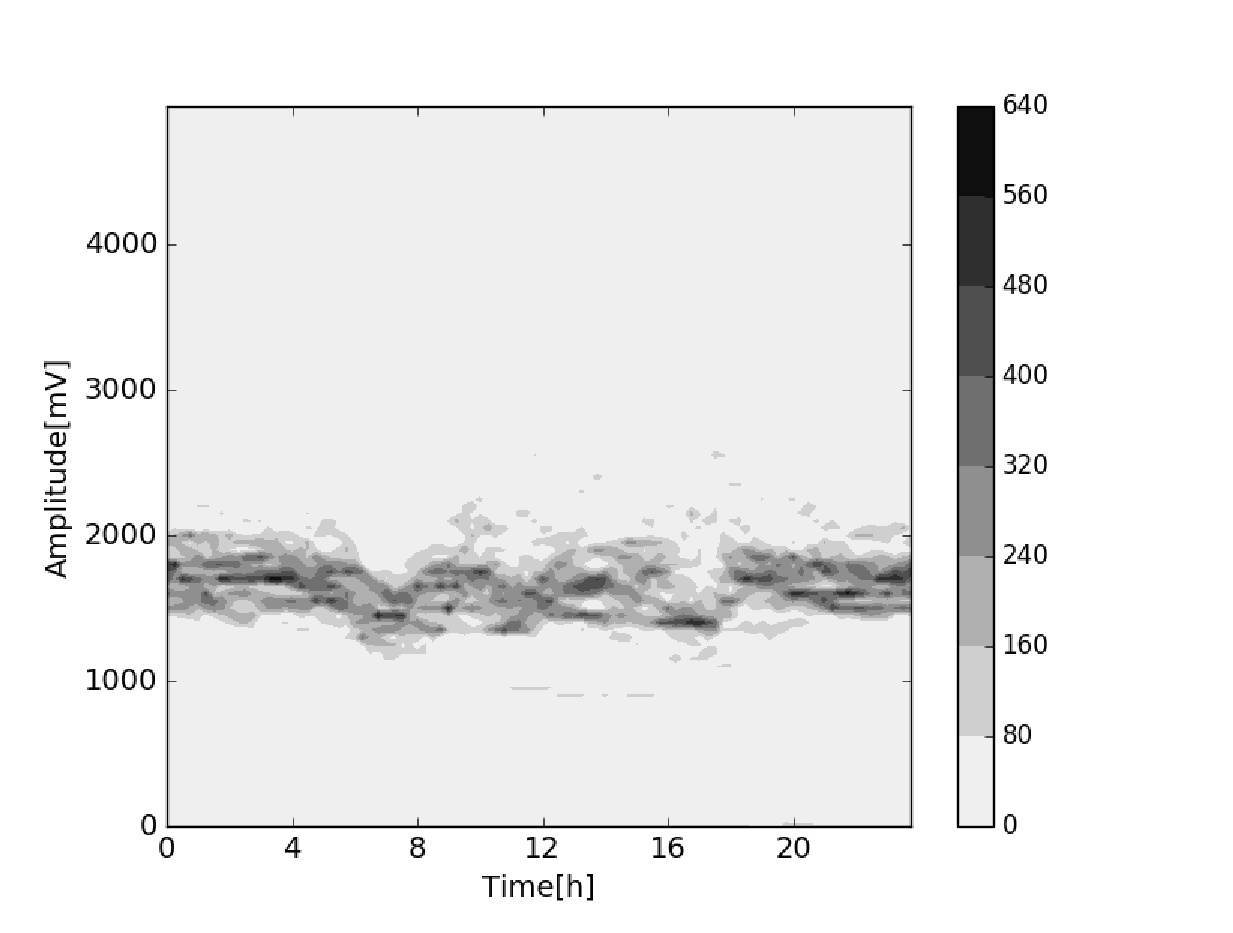
\includegraphics[width=10cm]{./fig/C_matrix.eps}
\caption{(JRMのFig.6)2週間分の排泄データを用いて作成した最頻値抽出行列}
\label{hist-spectrogram}
\end{figure}

各時刻において最頻値の違いが見られることから,最頻値抽出行列は被介護者の生活パターンを表していると考える.また,最頻値抽出行列は異常値を吸収できていると考えられるため,最頻値はベースラインを表している.\\
したがって,この最頻値の系列をk-meansでクラスタリングすることで,平常の場合の離床時と着床時のガスセンサ値のクラスタを見つけることができ,これを用いることで離着床判定可能である.\\
また,このとき重心が大きい値を取るクラスタを着床時のもの,重心が小さい値を取るクラスタを離床時のものとした.\\
ここで,重心とは各クラスタにおける平均ベクトルのことである.以下,最頻値を用いた離着床判定の手続きを以下に示す.

\begin{enumerate}
\item 滑走窓によって部分時系列に分割された排泄データが入力される
\item 窓中の値がk-meansによってあらかじめ分けたクラスタ二つのうちどちらに属しているか評価する
\item 窓内の「離床」クラスタに属すると評価された値が窓の1/3以下である場合は着床,そうでない場合は離床とする.
\end{enumerate}

排泄検知アルゴリズムI(以下,アルゴリズムI)における排泄検知部の簡易フローチャートを\refFigJp{cluster1}に示す.

\begin{figure}[t]
\centering
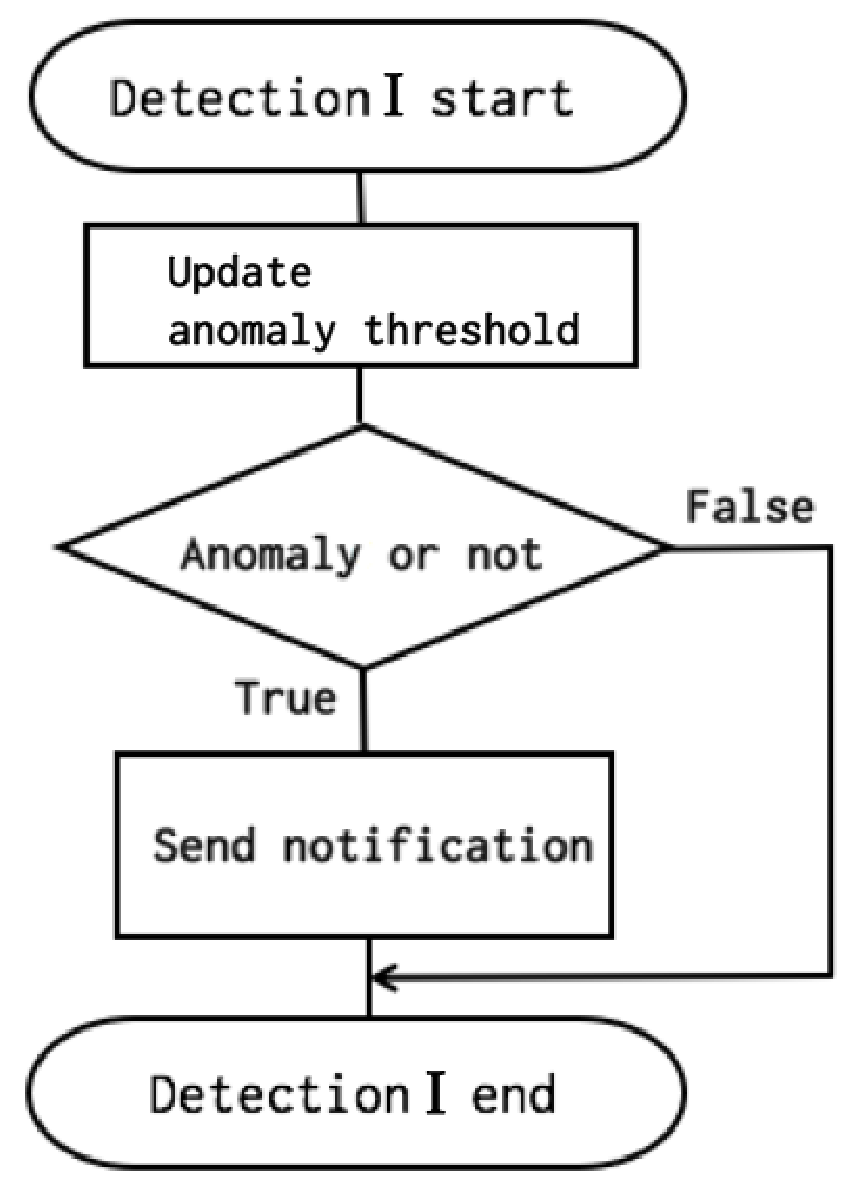
\includegraphics[width=5cm]{./fig/detection1.eps}
\caption{(JRMのFig.7)排泄検知部の簡易フローチャート}
\label{cluster1}
\end{figure}

アルゴリズムIは,滑走窓によって部分時系列になった排泄データに関しての値を逐一評価し,排泄を検知するアルゴリズムである.このときの評価には,離着床判定部のクラスタリングに基づいて決定される閾値を用いる.\\
離着床判定部では離床または着床のクラスタにクラスタリングされているが,これを異常値の判別にも利用した.\\
具体的には着床クラスタの重心から200[mV]以上上昇している区間が窓長の1/3を超えた場合,その滑走窓を異常値検出窓とした.\\
これらの値は以下のように経験値から決定されている.\\
数々の試行から二つのクラスタ間のセンサ出力値の差は,ほぼ400[mV]であった.\\
このことを用い二つのクラスタのうち着床クラスタの重心より両クラスタ間の1/2に相当する200[mV]を閾値とした.\\
また,窓長の1/3に関しては,各窓のどの位置からセンサ値が上昇を始めているのか,あるいは前の窓で上昇していたセンサ値がどの程度で下降していくかということを考えた場合,上昇,下降と変化なしの3状況が考えられることから1/3とした.\\
ちなみに,この1/3以上という条件を課すことによって放屁によるような突発的な異常値による誤検出も防げることが期待される.\\
すなわち,このアルゴリズムでは過去の排泄データを用いた教師なし学習によって閾値を決定することで個人に最適化させ排泄を検知する手法を用いている.

排泄検知アルゴリズムI\hspace{-.1em}I(以下,アルゴリズムI\hspace{-.1em}I)における排泄種類クラスタリング部の簡易フローチャートを\refFigJp{cluster2}に示す.

\begin{figure}[t]
\centering
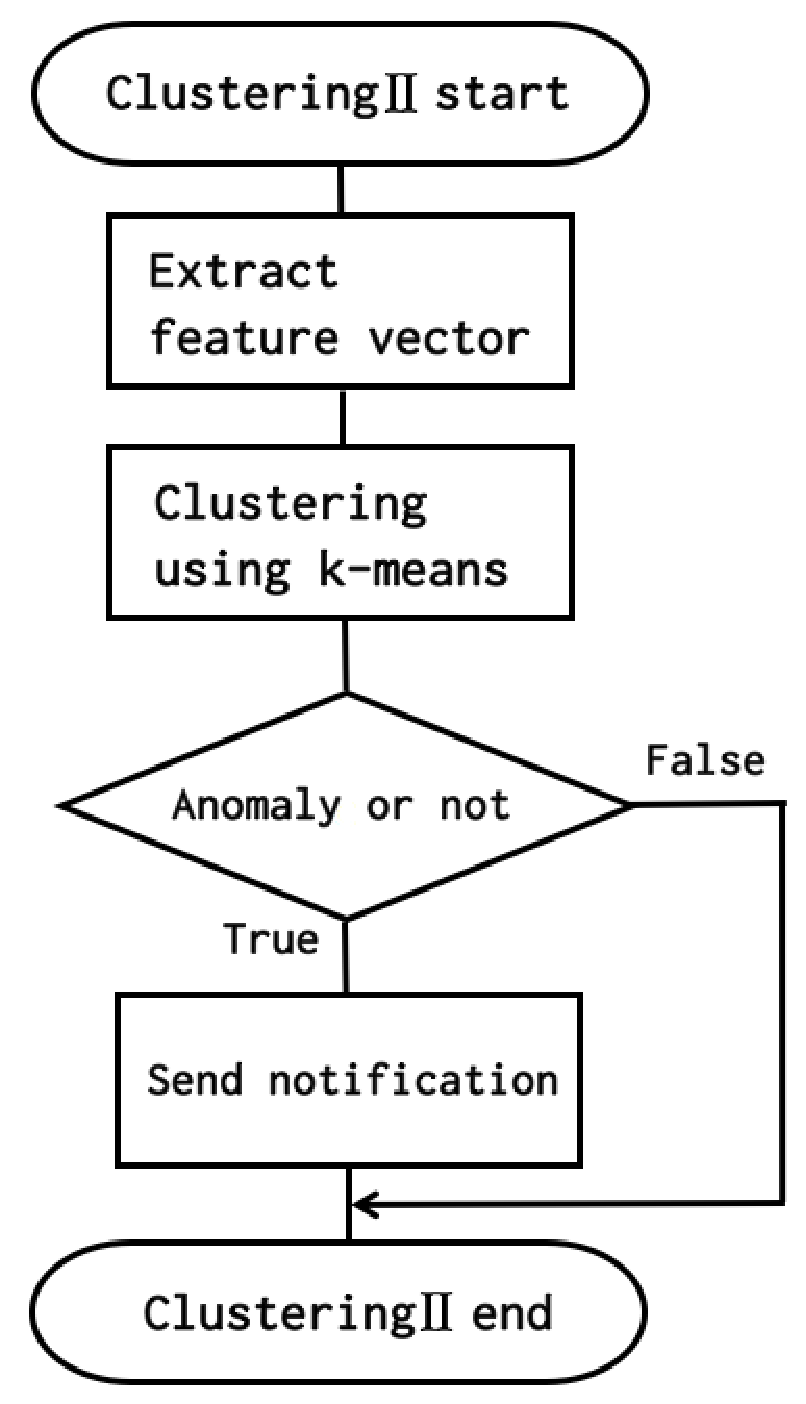
\includegraphics[width=5cm]{./fig/detection2.eps}
\caption{(JRMのFig.8)排泄種類クラスタリング部の簡易フローチャート}
\label{cluster2}
\end{figure}

アルゴリズムI\hspace{-.1em}Iでは,滑走窓から特徴量を抽出し,学習済みのk-meansモデルに入力することで,この滑走窓がどのクラスタに属するかを判断し,通知するかどうかと通知する内容を決定する.ここで,アルゴリズムI\hspace{-.1em}Iにおけるk-meansモデルは,クラスタ数3としている.この3というパラメータ値は,クラスタが{平常,排便,排尿}の三つに分かれることを期待して設定した.

k-meansモデルに入力する特徴量ベクトルは,滑走窓内で,一つ前の値との差分値を窓とした差分窓から抽出する標準偏差,最大値,最小値,正面積,負面積の5次元ベクトルである.標準偏差は,データのブレ具合を表しており,この値が大きい場合には異常であると言える.最大値,最小値は臭いの度合いを表していると考えられる.また,ここで正面積は窓中の正の値を積算した値であり,負面積は窓中の負の値を積算した値である.正面積は,正の差分値の積算値なため原波形の増加度に対応する.逆に,負面積は原波形の減少度に対応する.便臭は,尿臭と比べて臭源が個体であるため臭いの減衰が遅く,原波形の増加度や減少度によって切り分けできると考えられるため選択した.

\subsection{アルゴリズムの検証}\label{chap:3.3.3}
ほぼ寝たきりの高齢者という条件の被介護者を対象に,アルゴリズムIおよびI\hspace{-.1em}Iによる通知を行った.\\
期間は5週間であり,被験者10人を対象とし実験を開始した.10名全て女性で年齢は70歳後半から80歳後半であった.

アルゴリズムIの検証では,定時おむつ交換の際の排泄内容とアルゴリズムIによって通知された際の排泄内容の2種類のイベントデータも同時に記録した.
ただし,1日中イベントデータを記録することは不可能であるため,被験者が着床している19時から翌朝6時までの間に限定し実施した.
なお,実験時の詳細な手順については,Appendix?を参照されたい.

また,システムの通知の評価を正報,失報,誤報と以下のように定義する.

\begin{description}
\item[正報] システムが通知し,実際に排泄があった場合.
\item[失報] 排泄はあったもののシステムが通知することができなかった場合.
\item[誤報] システムが通知したものの,実際には排泄がなかった場合.
\end{description}
\par

また,このうち失報には,以下に示すような大きく2通りのパターンがあると考えられる.

\begin{description}
\item[ハードウェア的エラー] 結露による水つまりなどにより排泄臭を吸引できないなどハードウェアに起因する要因で排泄データに特徴が現れない場合
\item[ソフトウェア的エラー] 排泄データは得られているがイベントを予測できなかった場合
\end{description}
\par

すなわち,ソフトウェア的に回避が不可能なエラーが存在するため,実験の結果の評価はあくまでアルゴリズムのものではなく,システム全体のものとしておこなう.それに対して,ハードウェア的エラーの影響には大小あることが考えられるが誤報は一貫してソフトウェア的エラーとする.収集したデータ数は802件であった.
以下に実験時の詳細な手順を記載する.

アルゴリズムI\hspace{-.1em}Iの検証では,
\refFigJp{event}に示すように排泄データ中に二つの隣り合ったおむつ交換(図中のイベントX 及びY)が記録されていたとする.

\begin{figure}[t]
  \centering
  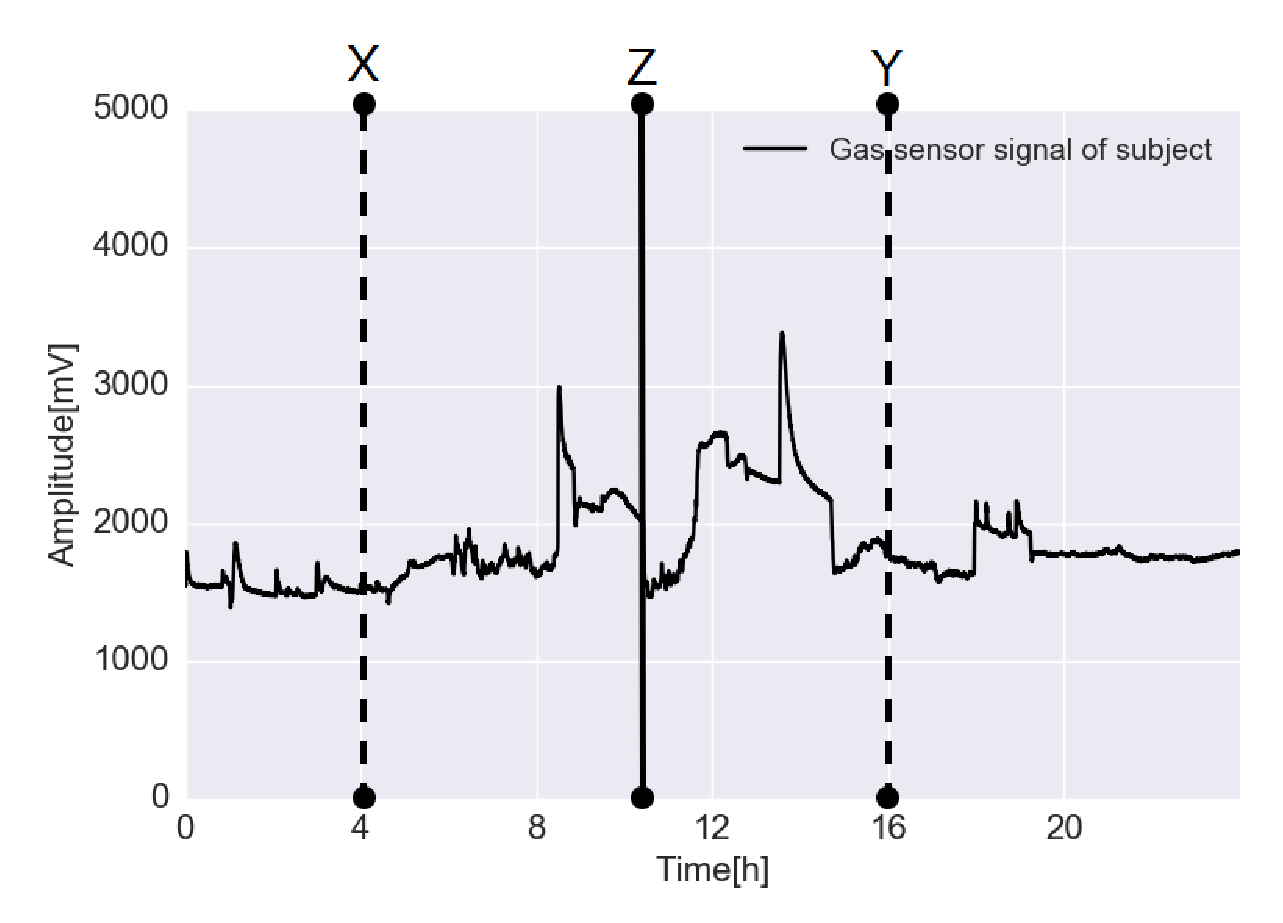
\includegraphics[width=8cm]{./fig/xyz.eps}
  \caption{(JRMのFig.9)排泄データとおむつ交換記録}
  \label{event}
\end{figure}

この時おむつ交換 Y の時点での排泄報告(あり,なし) と,両おむつ交換の間に検出された結果(あり,なし)とが合致していた場合を正報,報告が排泄ありで検出がなしの場合を失報,報告がなしで検出が排泄ありであった場合を誤報とする.このとき,実験に使用する排泄データは,アルゴリズムⅠの検証で用いるデータの最終1週間とし,イベントデータはその際に記録されたものを使用する.k-meansモデルの学習は,検知実験に用いる1週間の排泄データと同じ被験者から収集した2週間分の排泄データを使用する.このとき,排泄データ取得実験の第 5 週の排泄検知結果と比較して,正報や失報の回数がどのように変化するか調査した.

\subsection{アルゴリズムの検証結果}\label{chap:3.3.4}
アルゴリズムIの検証では,10人で行った実験において,実験協力者が実験機に不慣れであったための破損及び被介護者の体調不良に起因する便漏れによるシートの汚染などのケースが重なり計4名分のデータに不備が生じた.\\
また,体調を崩して入院し施設からいなくなった被介護者も1名いたため,合計5名に関して実験継続が不可能となった.\\
したがって,アルゴリズムの検証用には残り5名のデータを用いた.

今後,被験者A,B,C,D,Eとする.\refTblJp{notification1}に5週間の排泄検知結果を示す.

% table 1
\begin{table*}[t]
\begin{center}
\caption{(JRMのTable1)5週間の排泄検知結果}
\begin{tabular}[t]{c|r|r|r|r|r}
\hline
Name of examinee & 1st week [\%] & 2nd week [\%] & 3rd week [\%] & 4th week [\%] & 5th week [\%] \\ \hline
A & 16.6 & 0 & 52.3 & 52.9 & 0 \\ \hline
B & 30.0 & 25.2 & 66.7 & 67.7 & 61.5 \\ \hline
C & 52.6 & 60.0 & 44.4 & 42.9 & 47.4 \\ \hline
D & 42.1 & 55.6 & 33.3 & 41.2 & 37.5 \\ \hline
E & 33.3 & 63.6 & 50.0 & 54.5 & 33.3 \\ \hline
\end{tabular}
\label{notification1}
\end{center}
\end{table*}

ここで,排泄検知率は以下の計算式により求めた.

\begin{eqnarray}
  \mbox{排泄検知率}=\frac{\mbox{正報の回数}}{\mbox{(正報,誤報,失報の回数の和)}} \label{exec}
\end{eqnarray}
\par

また,\refTblJp{inout_table}に,実験期間のうちk-meansに入力する排泄データの収集が十分できた状態で行った最後の2週間の離着床判定の評価結果を示す.

% table 2
\begin{table*}[t]
\begin{center}
\caption{(JRMのTable 2)2週間の離着床判定の評価結果}
\begin{tabular}{c|ccc|ccc}
\hline
\multicolumn{1}{l|}{\shortstack{\\Name of\\examinee} } & \multicolumn{3}{l|}{Judgement rates in 4th week [\%]}                                  & \multicolumn{3}{l}{Judgement rates in 5th week [\%]}                                 \\ \cline{2-7} 
\multicolumn{1}{l|}{}                                & \multicolumn{1}{c|}{Total} & \multicolumn{1}{c|}{In-bed} & \multicolumn{1}{c|}{Out-of-bed} & \multicolumn{1}{c|}{Total} & \multicolumn{1}{c|}{In-bed} & \multicolumn{1}{c}{Out-of-bed} \\ \hline
A & 71.9 & 87.6 & 37.9 & 70.5 & 92.3 & 14.8 \\ \hline
B & 84.1 & 85.0 & 81.8 & 69.8 & 62.0 & 71.6 \\ \hline
C & 83.5 & 94.0 & 56.8 & 86.5 & 98.1 & 56.8 \\ \hline
D & 91.0 & 98.2 & 61.5 & 85.6 & 99.7 & 42.3 \\ \hline
E & 56.1 & 61.0 & 43.7 & 77.7 & 98.3 & 31.3 \\ \hline
\end{tabular}
\label{inout_table}
\end{center}
\end{table*}

ここで,全体判定率,着床判定率,離床判定率は以下のように求めた.また,判定結果が眠りSCANデータと一致しているものを正答としている.

\begin{eqnarray}
  \mbox{全体判定率}&=&\frac{\mbox{正答したデータ点数}}{\mbox{全体のデータ点数}} \label{all}\\
  \mbox{着床判定率}&=&\frac{\mbox{着床を正しく判定した点数}}{\mbox{実際に着床していた点数}} \label{bedin}\\
  \mbox{離床判定率}&=&\frac{\mbox{離床を正しく判定した点数}}{\mbox{実際に離床していた点数}} \label{bedout}
\end{eqnarray}
\par

\refTblJp{notification1}に示したように,個人差や各週における違いが非常に大きかった.また,被験者Aに関してはハードウェア的エラーや排泄臭が極端に弱いなどの理由により波形に特徴的パターンがほとんど現れず,0\%の週もあった.このようなことが排泄検知実験における実験環境のコンディションや個人に適応させていくことの難しさの一つである.一方で,被験者Bでは閾値を学習することにより6割台の検知率に上昇しており,比較的成功したケースであるといえる.

また,\refTblJp{inout_table}に示した離着床判定の結果を見ると,全体として着床判定率は低くても60\%台であり,ほとんどの場合で80\%以上を超えている.そのため,生活パターンに着目した最頻値抽出行列は着床の有無判断に対して有用であると考える.一方,離床判定率は個人差が大きかった.これは離床しているのにも関わらず,着床していると判断している場合が多いということである.これは,離床時にはベッド周辺の臭いに大きく影響されてしまっていたことが考えられる.一方で,着床時にはベッドに被介護者が乗り,掛け布団などをかけるため比較的安定した値が測定されたため判定率が高いと考えられる.
したがって,離床時にベッド周辺の臭いに影響されてしまうガスセンサだけでは,これ以上離床判定率を上げることは難しい.
よって,湿度センサを利用するなどして情報量を増やすことで離床判定率の向上を考える.しかし,離着床判定としては十分な精度であるといえ,排泄検知部に与える影響は少ないと考えられる.

アルゴリズムI\hspace{-.1em}Iの検証では,実験の結果は\refTblJp{notification2}のようになった.

% table 3
\begin{table}[t]
\begin{center}
\caption{アルゴリズムI\hspace{-.1em}Iの検証}
\begin{tabular}[t]{c|r|r}
\hline
\shortstack{\\Name of\\examinee} & \shortstack{\\Excretion detection\\rate of\\entire system [\%]} & \shortstack{\\Excretion detection\\rate of\\algorithm only [\%]}  \\ \hline
A & 30.8 & 100.0  \\ \hline
B & 65.0 & 65.0  \\ \hline
C & 35.7 & 62.5  \\ \hline
D & 20.0 & 62.5  \\ \hline
E & 42.8 & 66.7  \\ \hline
\end{tabular}
\label{notification2}
\end{center}
\end{table}

この表におけるシステム全体の排泄検知率は\refEqJp{exec}によって計算されるものであり,実験において現れたすべての失報を考慮した排泄検知率であり,ハードウェアとソフトウェアを含むシステム全体の検知率である.それに対し,アルゴリズムのみの排泄検知率はアルゴリズム自体の性能を評価するため,ハードウェアが原因とみなされる状況,すなわちガスセンサ値の変動がほとんど認められない部分を除いたデータを作り,それらを用いて\refEqJp{exec}によって検知率を計算したものである.
また,この計算に用いたデータはハードウェアの問題点と推測されるものを人為的に削除したデータを用いた解析であるため,単純な検出率のみ算出している.

\refTblJp{notification1}の第5週のカラムの結果と\refTblJp{notification2}のシステム全体の排泄検知率を比べると性能としてほとんど変わらない結果となった.ソフトウェア的に精度を上げることが困難であることが考えられたため,失報が起きている箇所の波形を実際にプロットし,ソフトウェア的エラーによる失報なのかハードウェア的エラーによるものなのか調査を行った.結果として,ほとんどの失報箇所において排泄データに特徴的なパターンが見られず,フラットな波形であった.したがって,チューブの水詰まりなどの要因によってセンサが測定できていなかった可能性が考えられる.

ソフトウェア的には,窓長やクラスタ数の変更によって結果が異なるため,研究を継続によって排泄検知に適したパラメータ値を見極める必要があると考える.

さらに,特徴的なパターンが現れるものの排泄はない場合に起こる誤報を無くす事が必要である.このような誤報は,多くは放屁によるものであると考えられ,切り分けるためには,放屁とその他の排泄波形パターンそれぞれを切り分け得る特徴量を検討することやクラスタ数の変更によって対応することが必要である.

\subsection{製品版としてのアルゴリズムの改良}\label{chap:3.3.5}
本研究では,ガスセンサによる離床判定を取り入れたが,製品にアルゴリズムを組込む場合,最頻値抽出行列を演算することはハードウェアのスペック的に困難であると言える.また,窓長やクラスタ数の変更によって結果が異なるため,排泄検知に適したパラメータ値の発見が十分ではないため,製品版では離床判定を抜いたアルゴリズムを用いることとした.\\
また,アルゴリズムの処理部分をハードウェア内ではなく,クラウド環境にすることにより,様々な場所や利用者の排泄データの取得が実現できると考えた.さらに,排泄をユーザに通知し,まだ十分な方法を考慮できてないないが排泄結果の情報を教師データとすることで,ビックデータとも言えるデータ郡を利用して,より精度を向上させたパラメータ値の探索が行えると考えている.\\
蓄積したデータを基に定期的にパラメータを更新することによって検知率は向上し,更には個々人に合わせたパラメータ値の探索なども可能であると考える.

★
\begin{figure}[htbp]
   \centering
   
\includegraphics[width=5cm]{./fig/temp.eps}
   \caption{実験時に取得した高齢者の波形データ(全て同一人物)}
   \label{mic17a}
\end{figure}

★
\begin{figure}[htbp]
   \centering
   
\includegraphics[width=5cm]{./fig/temp.eps}
   \caption{若者と高齢者におけるセンサ波形の違い}
   \label{mic17a}
\end{figure}
=======
%3.3
\section{アルゴリズムの構築}\label{chap:3.3}
この節では,排泄検知に関する関連製品とそれらのアルゴリズムの概要ならびに
本研究におけるアルゴリズム構築および検証について述べる.


\subsection{排泄検知に関する関連製品とアルゴリズムの概要}\label{chap:3.3.1}
まずはじめに,他の排泄検知に関する関連製品がどのような方法を用いて検知しているか述べる.
筒口ら(参考文献)は,排便後の早急なおむつ交換を可能とするため,高齢者や障害者の排便を検知するセンサシステムの開発と臨床現場での評価試験をおこなった.
このセンサシステムには,硫化水素,アミン系,VOC(有機揮発物質)の3種類に反応するガスセンサ3つと温度センサを採用している.
おむつにはチューブと温度センサが設けられており,チューブからおむつ内の空気を吸引することによってにおいを計測するとともに,温度センサによっておむつ内の温度を計測する.
この合計4つのセンサ値を処理することによって排便検知をおこなう.実験により,各センサによって計測されるデータの傾向を示した.\par
しかし,複数の化学物質に反応するような選択性のないガスセンサと比較して,硫化水素やアミン系など特定の化学物質に対して選択性を持っているガスセンサは高価である.
そのため,製品化を考えている場合には採用することが難しい.
また,おむつ内に温度センサを載せておくことやチューブを挿しておかなければならないことから,被介護者の体にデバイスが接触することによる不快感や危険性か存在すると考えられる.\par

他にも,水川ら[6]は,FIGARO技研株式会社製のガスセンサTGS2450をおむつに装着した排泄検知システムを提案している.
おむつに装着するため装着時の違和感を軽減するために小型であることと,センサが汚染された場合には廃棄できるように安価であることを条件として選定している.
水川らは,TGS2450に関する応答時間や加熱時間特性などに関する実験をおこない,ガスセンサを用いた排尿・排便検知が十分可能であることを示した.
このように,ガスセンサを用いた排泄検知に関する研究や製品は散見される.しかし,おむつに装着する必要があるため,違和感や不快感が伴う場合があると考えられる.
また,センサを廃棄する場合も多く,コスト面の問題も考えられる.一方で,排泄部周辺の空気を吸引することでセンサ値を取得する製品も見られる.
フォーリーブス株式会社は,尿や便を吸引パイプで吸引しガスセンサによって検出するシステムを開発した[b].
防水フィルタを施したポンプによって吸引するため汚染されない仕組みをとっており,アルゴリズムによっておならを検出することもできる.
排便と排尿の識別にはベースラインからのピークの幅の違いを用いており,非接触型となっている.
後述する本研究のアルゴリズムもこのシステムと同様に,排泄部周辺の空気を吸引することで排泄検知を実現しているが,ガスセンサ値にはセンサ個体差や利用者の個人差によるばらつきが大きいため,それらを吸収するアルゴリズムを備えている点が異なる.\par

次に,排泄検知システムにおけるアルゴリズムについて述べる.ここでのアルゴリズムとは,センサデータを用いて排泄検知を可能とするソフトウェア処理手順を指す.
これまでに製品化された排泄検知製品は,そのハードウェア構造によりある程度であるがアルゴリズムの処理概要を推測することが可能であり,大きく分けて以下の2種類のグループに分類が可能であると考えた.
\begin{enumerate}
\item センサの出力値が2値(1と0,5Vと0V,など)となるものを用いて出力値の状態を基に判断する方法
\item センサが取得する物理量(空気中のガス濃度や温度,湿度など)が決められた一定の値(閾値)に達するか否かを判断する方法
\end{enumerate}
\par


1つ目の方法では,接点スイッチや濡れセンサ(水などの液体による通電を接点とするもの)ような部品を使用していることが多く見受けられる.
ハードウェアとしても単純な構造となり,アルゴリズムとしても「1」であるか「0」であるかという簡易な条件分岐のみで良いため複雑な処理の必要がない.
{\color{red}【例えば,ある製品ではおむつ内に濡れセンサを用いることによって排泄時(特に尿)を検知することが可能である.】}
しかし,対象事象が特定の2値状態で分類可能であることやそれらの状態の境界を自由に決定できない事があり,
濡れセンサなどは一度反応するとその状態を維持してしまうことなどもあるため,リセットや使い捨てによる交換など何らかの対応が必要となる事がある.
また,0と1の間の0.5のようなファジィな状態を持つ対象には不向きである.
{\color{red}【前述の例では,濡れセンサが使い捨てとなっており,交換が必要である.】}\par
2つ目の方法では,利用するセンサの取得可能な値域(レンジ)内に任意で基準を設ける(複数可)ことが可能であり,その基準値に従って条件分岐が可能であるため,設計者が任意の値を対象状態の境界に設定することが可能である.
{\color{red}【例えば,VOCなどに反応するガスセンサと温度センサを利用したある製品では,ある温度Tとセンサ値Cを処理し,放屁または排便(排尿)を検知することが可能である.】}
しかし,利用するセンサの個体差やセンサ値を算出する際の分解能などハードウェアに依存してしまう部分や対象の状態が無数に存在することによるユニークな閾値決定の困難さなどが存在し,
結果的にアルゴリズムの複雑化を起こし,処理時間の増加などの原因となる.
{\color{red}【前述の例では,設計者が決定したTやCの閾値が対象状態の実際の境界値ではない可能性があることが挙げられる.】}


\subsection{本研究におけるアルゴリズム構築}\label{chap:3.3.2}
本研究におけるアルゴリズムは,実際の現場へ導入することを目的としていたため,1つのアルゴリズムで多人数に対応可能である必要があった.
しかし,使用するTGS2602\footnotemark[1]はセンサ自身に個体差を持っており,その差は比較的大きいものであった.
較正(キャリブレーション)することも考慮したが,個人の排泄臭にも大きな差が生じる知見があったため,簡易的なものでは吸収が困難であると判断し,教師データを用いた機械学習に着目した.
初期の段階で健常者による研究室データを用いた実験[松本卒論]では,ある程度安定した波形かガスセンサから得られていたため,波形の局所的な特徴を用いていた.
また教師データとなる正解は常に記録されていたため,教師付き学習を用いることが容易であった.
しかし,介護施設における実際のデータに関してはセンサ波形のバリエーションが多かったため,局所的な情報の使用を断念し,大局的な特徴量を用いることとした.
また,実際の介護現場ではガスセンサの応答に対して正解を記録する作業が,非常に困難であることがわかり,教師付きのデータの取得を断念した.
本アルゴリズムでは,排泄データの部分時系列データをk-means法によって教師なしで排泄検知と排泄種類判別をおこなっている.
\footnotetext[1]{フィガロ技研株式会社の製品である空気の汚れ・ニオイ検知用ガスセンサ.空気の汚れ(VOC,アンモニア,硫化水素など)を検知対象としている.}

排泄検知アルゴリズムの概要フローチャートを\refFigJp{algo_flow}に示す.
\begin{figure}[t]
\centering
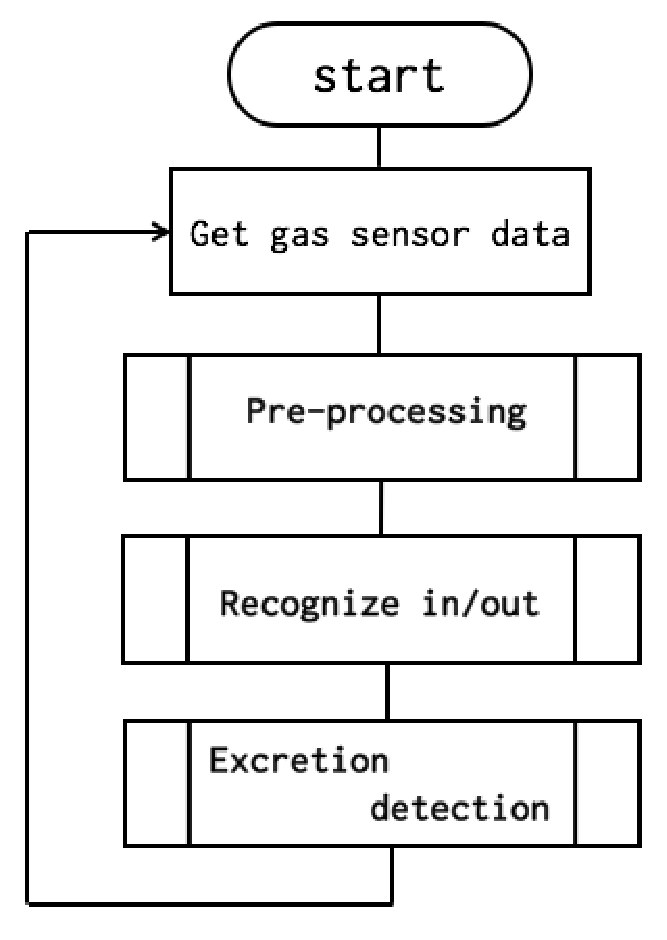
\includegraphics[width=5cm]{./fig/algoflow.eps}
\caption{Overall flow chart of the excretion detection algorithm.}
\label{algo_flow}
\end{figure}

本研究で採用している排泄検知アルゴリズムは,大きく分けて以下の3つである.
\begin{itemize}
\item 前処理部
\item 離着床判定部
\item 排泄検知部
\end{itemize}
\par

本研究では排泄検知部を2つ考え評価するものとする.
ここで,その2つを排泄検知部I,I\hspace{-.1em}Iと名付けることとし,それらを採用した排泄検知アルゴリズムを排泄検知アルゴリズムI,I\hspace{-.1em}Iとする.
すなわち,3つの処理のうち前処理部と離着床判定部は共通であり,排泄検知部のみが異なる.以下,詳しく説明する.

前処理部では,排泄データの移動平均をとり平滑化することを行う.
排泄によるガスセンサの応答は,立ち上がりを見せて再度落ち着くまで約1,2時間程度を要する制限が存在するため,瞬間的な波形の特徴パターンよりは比較的長時間の特徴パターンによって十分クラスタリングできると考えた.
これまで知見から50秒の移動平均が最も適しているという結果を得ているが,区切りの良さと影響の程度を考慮した上で,1分の移動平均を取ることとした.
また,本アルゴリズムはこの移動平均値を15分単位の部分時系列データに分割された一つの窓として離着床,排泄検知に使用する.この窓のことを滑走窓と本研究では呼ぶ.

離着床判定部では,利用者がベッド上に存在するかどうかを判定する.
過去において利用者が着床していない場合でも,ベッド付近の排泄臭以外に反応して通知してしまうことがあった.
そこで,離着床判定を取り入れることによって利用者が離床しているのにもかかわらず通知してしまう誤報を減らすことを目的とした.
ここで正解率の高い離着床センサを併用することは,排泄検知をより正確にすることに貢献する.
しかし,開発しているハードウェアは市販を目的としており,その利用に関してのコストを最小化することは大きな要求であった.
その観点から,他の離床センサを使用することなく,現在使用しているセンサのみで離着床が判断できれば製品としての優位性が増すと考えた.
よって,本研究ではガスセンサによる離床判定を取り入れた.

\begin{figure}[t]
\centering
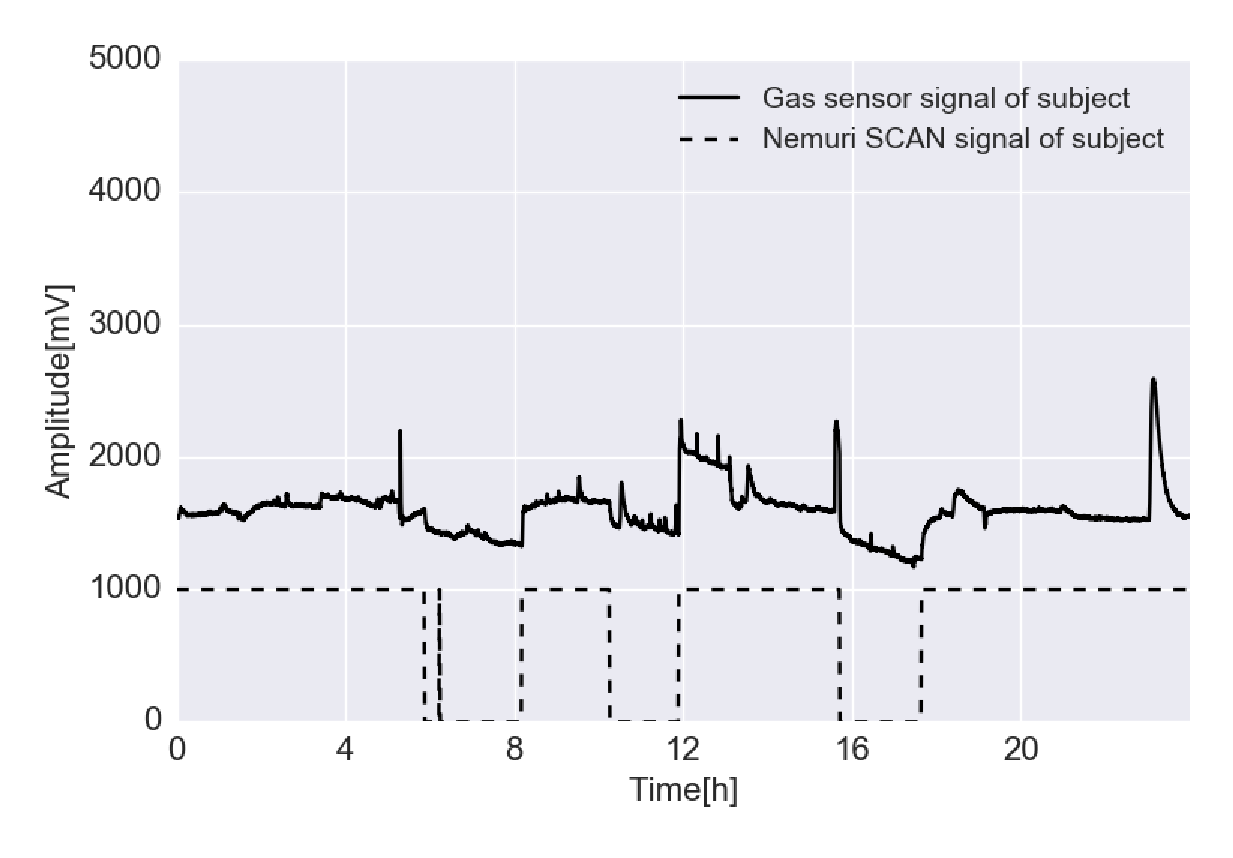
\includegraphics[width=8cm]{./fig/inout3.eps}
\caption{Comparison between excretion and Nemuri SCAN data.}
\label{inout3}
\end{figure}

\refFigJp{inout3}に移動平均によって平滑化した排泄データとパラマウントベッド株式会社の眠りSCANのデータを同時にプロットした例を示す.
2つのデータは,それぞれのデータに記されているタイムスタンプをもとしている.
ここで,眠りSCANはマットレスの下に敷くだけで睡眠状態の評価をすることができるデバイスである.
眠りSCANは離着床データを出力することができるため,離着床判定部の評価に用いることができると考えた.
\refFigJp{inout3}を見てわかるように,排泄データが離着床に応じて変化していることがわかったため,排泄データのベースラインを抽出することで,ガスセンサを用いて離着床判定を行うことができると考えた.
しかし,前述したようにTGS2602には個体差が存在し,個人の排泄臭や体臭の違いによる影響によって離着床時のベースライン値にばらつきが存在した.
また,ベースラインを抽出できても排泄によるデータ変動により単純にベースラインだけで離着床を識別することは困難であった.
そこで,被介護者の生活パターンに着目し,各時間帯における最頻値を統計的に抽出することで離着床判定をおこなうことを考えた.
本研究では各時刻において頻出して測定されるガスセンサ値を最頻値と呼ぶ.
さらに,まるでスペクトログラムのように横軸を時間,縦軸にガスセンサ値,ヒストグラムの度数を色で表示されるように並べたものを最頻値行列と定義した.
その際のフレーム幅やヒストグラムのビン幅は試行を経て算出した経験則値として900[s],50[mV]とした.


\begin{figure}[t]
\centering
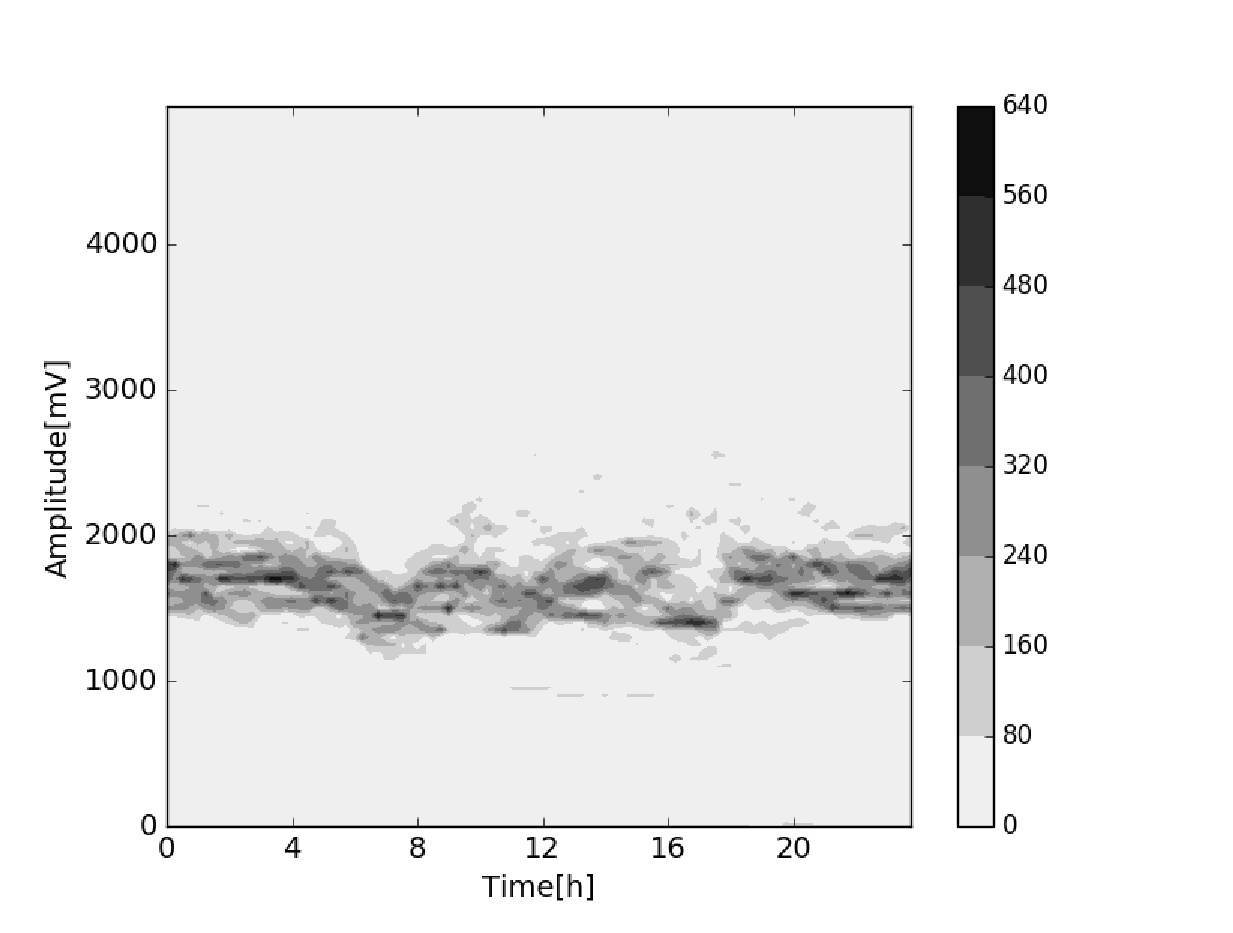
\includegraphics[width=10cm]{./fig/C_matrix.eps}
\caption{Example of mode extraction matrix created by placing histograms along the time axis.}
\label{hist-spectrogram}
\end{figure}

2週間分の排泄データを用いて作成した最頻値抽出行列の例を\refFigJp{hist-spectrogram}に示す.
各時刻において最頻値の違いが見られることから,最頻値抽出行列は被介護者の生活パターンを表していると考える.
また,最頻値抽出行列は異常値を吸収できていると考えられるため,最頻値はベースラインを表している.
したがって,この最頻値の系列をk-meansでクラスタリングすることで,平常の場合の離床時と着床時のガスセンサ値のクラスタを見つけることができ,これを用いることで離着床判定可能である.
また,このとき重心が大きい値を取るクラスタを着床時のもの,重心が小さい値を取るクラスタを離床時のものとした.
ここで,重心とは各クラスタにおける平均ベクトルのことである.以下,最頻値を用いた離着床判定の手続きを以下に示す.


\begin{enumerate}
\item 滑走窓によって部分時系列に分割された排泄データが入力される
\item 窓中の値がk-meansによってあらかじめ分けたクラスタ2つのうちどちらに属しているか評価する
\item 窓内の「離床」クラスタに属すると評価された値が窓の1/3以下である場合は着床,そそうでない場合は離床とする.
\end{enumerate}


\begin{figure}[t]
\centering
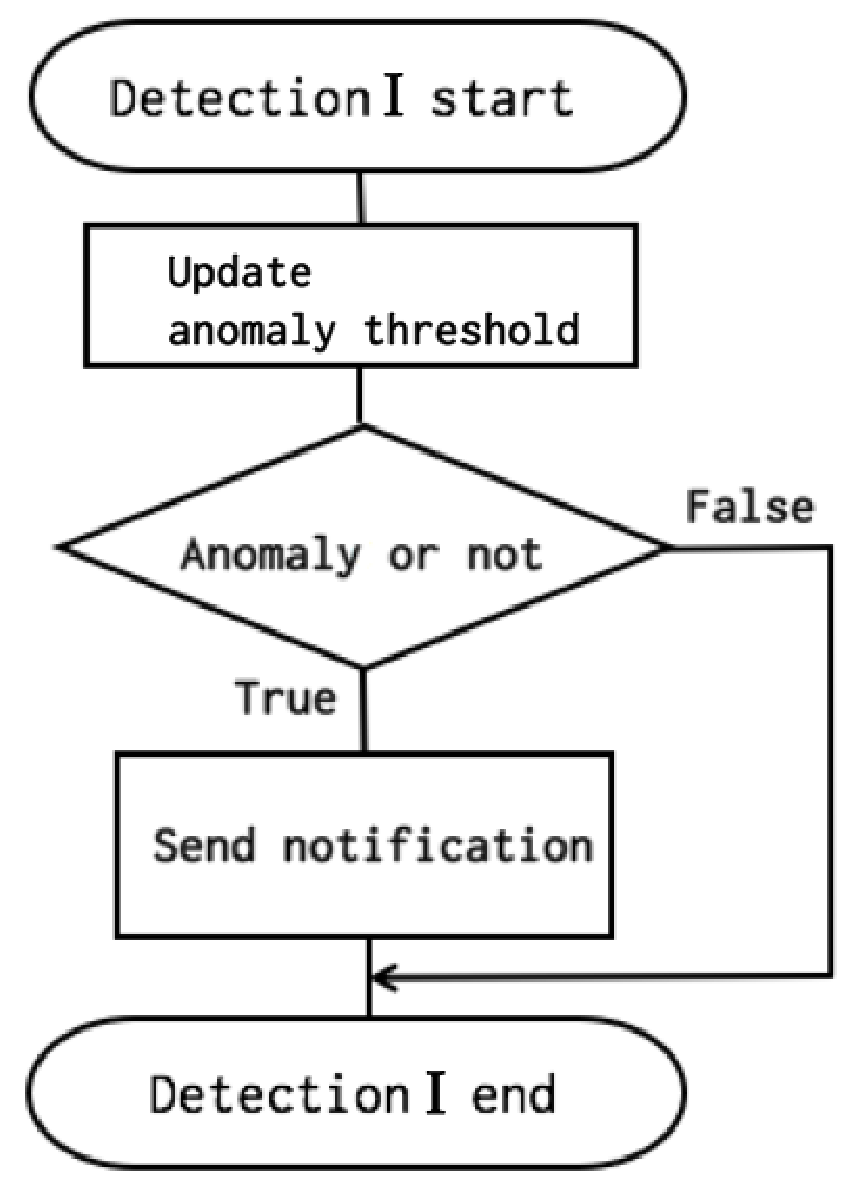
\includegraphics[width=5cm]{./fig/detection1.eps}
\caption{Algorithm I: Clustering by excretion type.}
\label{cluster1}
\end{figure}


\begin{figure}[t]
\centering
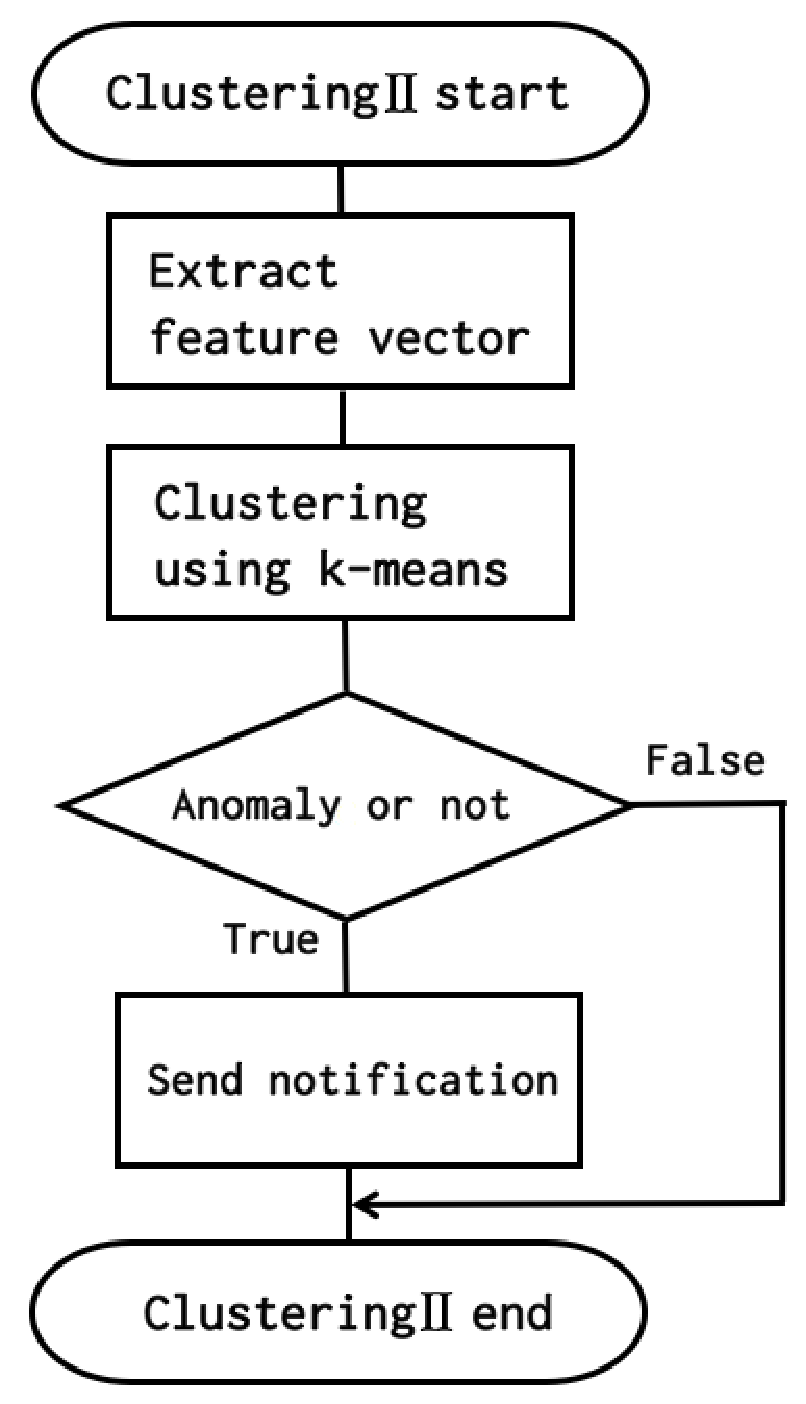
\includegraphics[width=5cm]{./fig/detection2.eps}
\caption{Algorithm I\hspace{-.1em}I: Clustering by excretion type.}
\label{cluster2}
\end{figure}

排泄検知アルゴリズムI(以下,アルゴリズムI)における排泄検知部の簡易フローチャートを\refFigJp{cluster1}に示す.
アルゴリズムIは,滑走窓によって部分時系列になった排泄データに関しての値を逐一評価し,排泄を検知するアルゴリズムである.
このときの評価には,離着床判定部のクラスタリングに基づいて決定される閾値を用いる.
離着床判定部では離床または着床のクラスタにクラスタリングされているが,これを異常値の判別にも利用した.
具体的には着床クラスタの重心から200[mV]以上上昇している区間が窓長の1/3を超えた場合,その滑走窓を異常値検出窓とした.
これらの値は以下のように経験値から決定されている.
数々の試行から二つのクラスタ間のセンサ出力値の差は,ほぼ400[mV]であった.
このことを用い2つのクラスタのうち着床クラスタの重心より両クラスタ間の1/2に相当する200[mV]を閾値とした.
また,窓長の1/3に関しては,各窓のどの位置からセンサ値が上昇を始めているのか,あるいは前の窓で上昇していたセンサ値がどの程度で下降していくかということを考えた場合,上昇,下降と変化なしの3状況が考えられることから1/3とした.
ちなみに,この1/3以上という条件を課すことによって放屁によるような突発的な異常値による誤検出も防げることが期待される.
すなわち,このアルゴリズムでは過去の排泄データを用いた教師なし学習によって閾値を決定することで個人に最適化させ排泄を検知する手法を用いている.

排泄検知アルゴリズムI\hspace{-.1em}I(以下,アルゴリズムI\hspace{-.1em}I)における排泄種類クラスタリング部の簡易フローチャートを\refFigJp{cluster2}に示す.
アルゴリズムI\hspace{-.1em}Iでは,滑走窓から特徴量を抽出し,学習済みのk-meansモデルに入力することで,この滑走窓がどのクラスタに属するかを判断し,通知するかどうかと通知する内容を決定する.
ここで,アルゴリズムI\hspace{-.1em}Iにおけるk-meansモデルは,クラスタ数3としている.
この3というパラメータ値は,クラスタが{平常,排便,排尿}の3つに分かれることを期待して設定した.

k-meansモデルに入力する特徴量ベクトルは,滑走窓内で,一つ前の値との差分値を窓とした差分窓から抽出する標準偏差,最大値,最小値,正面積,負面積の5次元ベクトルである.
標準偏差は,データのブレ具合を表しており,この値が大きい場合には異常であると言える.最大値,最小値は臭いの度合いを表していると考えられる.
また,ここで正面積は窓中の正の値を積算した値であり,負面積は窓中の負の値を積算した値である.正面積は,正の差分値の積算値なため原波形の増加度に対応する.
逆に,負面積は原波形の減少度に対応する.便臭は,尿臭と比べて臭源が個体であるため臭いの減衰が遅く,原波形の増加度や減少度によって切り分けできると考えられるため選択した.

\subsection{アルゴリズムの検証}\label{chap:3.3.3}
ほぼ寝たきりの高齢者という条件の被介護者を対象に,アルゴリズムIおよびI\hspace{-.1em}Iによる通知をおこなった.
期間は5週間であり,被験者10人を対象とし実験を開始した.被験者の個人情報は控えるが,10名全て女性で年齢は70歳後半から80歳後半であった.

アルゴリズムIの検証では,定時おむつ交換の際の排泄内容とアルゴリズムIによって通知された際の排泄内容の2種類のイベントデータも同時に記録した.
ただし,1日中イベントデータを記録することは不可能であるため,被験者が着床している19時から翌朝6時までの間に限定し実施した.
なお,実験時の詳細な手順については,付録\ref{chap:A}を参照されたい.
また,システムの通知の評価を正報,失報,誤報と以下のように定義する.

\begin{description}
\item[正報] システムが通知し,実際に排泄があった場合.
\item[失報] 排泄はあったもののシステムが通知することができなかった場合.
\item[誤報] システムが通知したものの,実際には排泄がなかった場合.
\end{description}
\par


また,このうち失報には,以下に示すような大きく2通りのパターンがあると考えられる.

\begin{description}
\item[ハードウェア的エラー] 結露による水つまりなどにより排泄臭を吸引できないなどハードウェアに起因する要因で排泄データに特徴が現れない場合
\item[ソフトウェア的エラー] 排泄データは得られているがイベントを予測できなかった場合
\end{description}
\par

すなわち,ソフトウェア的に回避が不可能なエラーが存在するため,実験の結果の評価はあくまでアルゴリズムのものではなく,システム全体のものとしておこなう.
それに対して,ハードウェア的エラーの影響には大小あることが考えられるが誤報は一貫してソフトウェア的エラーとする.収集したデータ数は802件であった.

\begin{figure}[t]
  \centering
  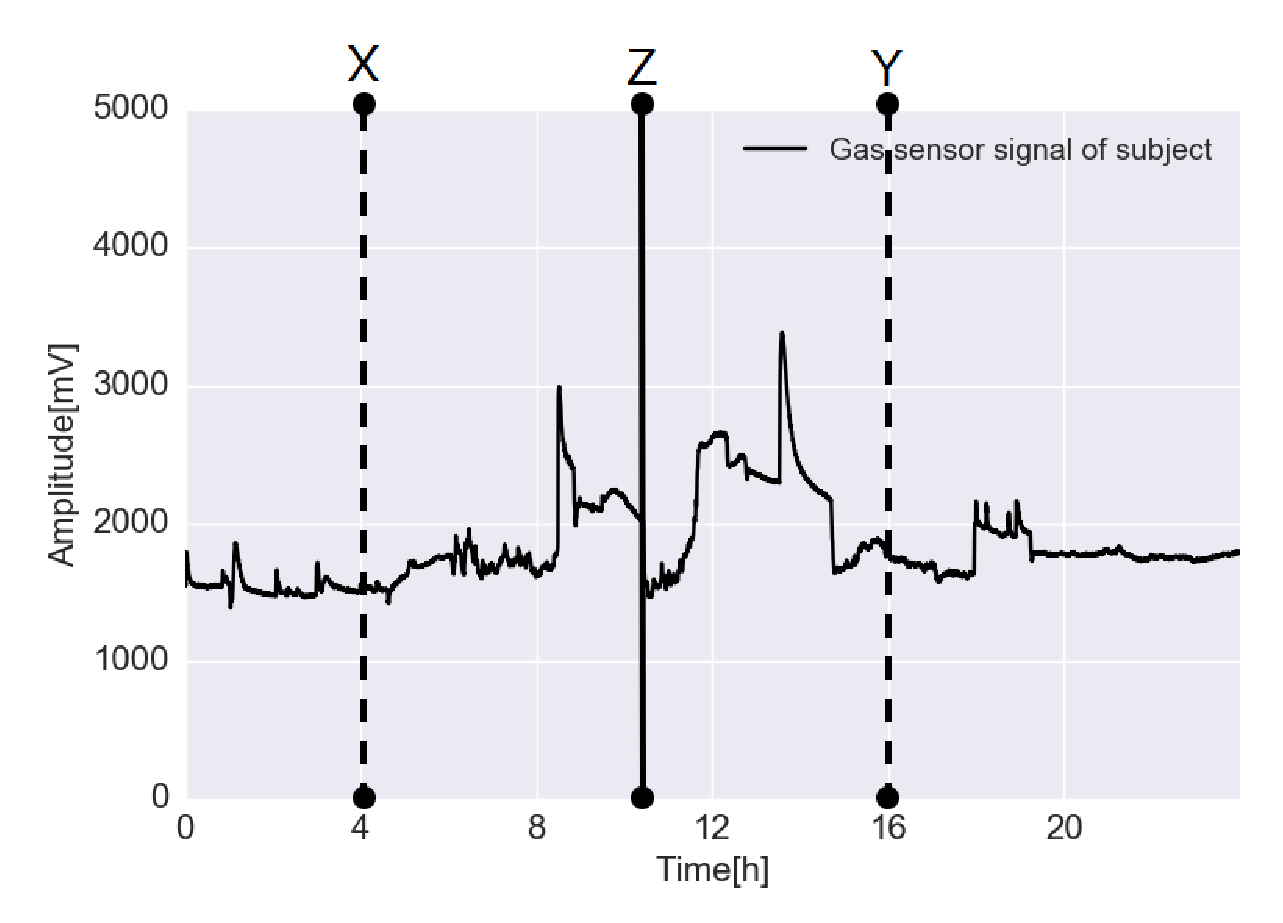
\includegraphics[width=8cm]{./fig/xyz.eps}
  \caption{Example of event X, event Y, and excretion detection Z}
  \label{event}
\end{figure}

アルゴリズムI\hspace{-.1em}Iの検証では,
\refFigJp{event}に示すように排泄データ中に二つの隣り合ったおむつ交換(図中のイベントX 及びY)が記録されていたとする.
この時おむつ交換Yの時点での排泄報告(あり,なし) と,両おむつ交換の間に検出された結果(あり,なし)とが合致していた場合を正報,
報告が排泄ありで検出がなしの場合を失報,報告がなしで検出が排泄ありであった場合を誤報とする.
このとき,実験に使用する排泄データは,アルゴリズムIの検証で用いるデータの最終1週間とし,イベントデータはその際に記録されたものを使用する.
k-meansモデルの学習は,検知実験に用いる1週間の排泄データと同じ被験者から収集した2週間分の排泄データを使用する.
このとき,排泄データ取得実験の第5週の排泄検知結果と比較して,正報や失報の回数がどのように変化するか調査を行った.


\subsection{アルゴリズムの検証結果}\label{chap:3.3.4}
アルゴリズムⅠの検証では、10人で行った実験において実験協力者が実験機に不慣れであったため,実験機器の破損や被介護者の体調不良などのケースが重なり計4名分のデータに不備が生じた.
また、体調を崩して入院し施設からいなくなった被介護者も1名いたため,合計5名に関して実験継続が不可能となった.
したがって,アルゴリズムの検証用データとして継続的に取得できた残り5名のデータを用いた.

% table 1
\begin{table*}[t]
\begin{center}
\caption{Excretion detection rate in the excretion data-acquisition experiment, using algorithm I}
\begin{tabular}[t]{c|r|r|r|r|r}
\hline
Name of examinee & 1st week [\%] & 2nd week [\%] & 3rd week [\%] & 4th week [\%] & 5th week [\%] \\ \hline
A & 16.6 & 0 & 52.3 & 52.9 & 0 \\ \hline
B & 30.0 & 25.2 & 66.7 & 67.7 & 61.5 \\ \hline
C & 52.6 & 60.0 & 44.4 & 42.9 & 47.4 \\ \hline
D & 42.1 & 55.6 & 33.3 & 41.2 & 37.5 \\ \hline
E & 33.3 & 63.6 & 50.0 & 54.5 & 33.3  \\ \hline
\end{tabular}
\label{notification1}
\end{center}
\end{table*}

% table 2
\begin{table*}[t]
\begin{center}
\caption{In-bed and out-of-bed judgment rates in excretion data-acquisition experiments with algorithm I}
\begin{tabular}{c|ccc|ccc}
\hline
\multicolumn{1}{l|}{\shortstack{\\Name of\\examinee} } & \multicolumn{3}{l|}{Judgement rates in 4th week [\%]}                                  & \multicolumn{3}{l}{Judgement rates in 5th week [\%]}                                 \\ \cline{2-7} 
\multicolumn{1}{l|}{}                                & \multicolumn{1}{c|}{Total} & \multicolumn{1}{c|}{In-bed} & \multicolumn{1}{c|}{Out-of-bed} & \multicolumn{1}{c|}{Total} & \multicolumn{1}{c|}{In-bed} & \multicolumn{1}{c}{Out-of-bed} \\ \hline
A & 71.9 & 87.6 & 37.9 & 70.5 & 92.3 & 14.8 \\ \hline
B & 84.1 & 85.0 & 81.8 & 69.8 & 62.0 & 71.6 \\ \hline
C & 83.5 & 94.0 & 56.8 & 86.5 & 98.1 & 56.8 \\ \hline
D & 91.0 & 98.2 & 61.5 & 85.6 & 99.7 & 42.3 \\ \hline
E & 56.1 & 61.0 & 43.7 & 77.7 & 98.3 & 31.3 \\ \hline
\end{tabular}
\label{inout_table}
\end{center}
\end{table*}


今後,被験者A,B,C,D,Eとする.\refTblJp{notification1}に5週間の排泄検知結果を示す.
ここで,排泄検知率は以下の計算式により求めた.

\begin{eqnarray}
  \mbox{排泄検知率}=\frac{\mbox{正報の回数}}{\mbox{(正報,誤報,失報の回数の和)}} \label{exec}
\end{eqnarray}
\par

また,\refTblJp{inout_table}に,実験期間のうちk-meansに入力する排泄データの収集が十分できた状態でおこなった最後の2週間の離着床判定の評価結果を示す.
ここで,全体判定率,着床判定率,離床判定率は以下のように求めた.
また,判定結果が眠りSCANデータと一致しているものを正答としている.

\begin{eqnarray}
  \mbox{全体判定率}&=&\frac{\mbox{正答したデータ点数}}{\mbox{全体のデータ点数}} \label{all}\\
  \mbox{着床判定率}&=&\frac{\mbox{着床を正しく判定した点数}}{\mbox{実際に着床していた点数}} \label{bedin}\\
  \mbox{離床判定率}&=&\frac{\mbox{離床を正しく判定した点数}}{\mbox{実際に離床していた点数}} \label{bedout}
\end{eqnarray}
 \par

\refTblJp{notification1}に示したように,個人差や各週における違いが非常に大きかった.
また,被験者Aに関してはハードウェア的エラーや排泄臭が極端に弱いなどの理由により波形に特徴的パターンがほとんど現れず,0\%の週もあった.
このようなことが排泄検知実験における実験環境のコンディションや個人に適応させていくことの難しさの1つである.
一方で,被験者Bでは閾値を学習することにより6割台の検知率に上昇しており,比較的成功したケースであるといえる.

また,\refTblJp{inout_table}に示した離着床判定の結果を見ると,全体として着床判定率は低くても60\%台であり、ほとんどの場合で80\%以上を超えている.
そのため,生活パターンに着目した最頻値抽出行列は着床の有無判断に対して有用であると考える.
一方,離床判定率は個人差が大きかった.これは離床しているのにも関わらず,着床していると判断している場合が多いということである.
これは,離床時にはベッド周辺の臭いに大きく影響されてしまっていたことが考えられる.
一方で,着床時にはベッドに被介護者が乗り,掛け布団などをかけるため比較的安定した値が測定されたため判定率が高いと考らえる.
したがって,離床時にベッド周辺の臭いに影響されてしまうガスセンサだけでは、これ以上離床判定率を上げることは難しい.
よって,湿度センサを利用するなどして情報量を増やすことで離床判定率の向上を考える.
しかし,離着床判定としては十分な精度であるといえ,排泄検知部に与える影響は少ないと考えられる.

アルゴリズムI\hspace{-.1em}Iの検証では、
実験の結果は\refTblJp{notification2}のようになった.
この表におけるシステム全体の排泄検知率は\refEqJp{exec}によって計算されるものであり,実験において現れたすべての失報を考慮した排泄検知率(ハードウェアとソフトウェアを含むシステム全体の検知率)である.
それに対し,アルゴリズムのみの排泄検知率はアルゴリズム自体の性能を評価するため、ハードウェアが原因とみなされる状況、すなわちガスセンサ値の変動がほとんど認められない部分を除いたデータを作り、それらを用いて\refEqJp{exec}によって検知率を計算したものである.
また,この計算に用いたデータはハードウェアの問題点と推測されるものを人為的に削除したデータを用いた解析であるため,単純な検出率のみ算出している.

% table 3
\begin{table}[t]
\begin{center}
\caption{Excretion detection rate in algorithm I\hspace{-.1em}I}
\begin{tabular}[t]{c|r|r}
\hline
\shortstack{\\Name of\\examinee} & \shortstack{\\Excretion detection\\rate of\\entire system [\%]} & \shortstack{\\Excretion detection\\rate of\\algorithm only [\%]}  \\ \hline
A & 30.8 & 100.0  \\ \hline
B & 65.0 & 65.0  \\ \hline
C & 35.7 & 62.5  \\ \hline
D & 20.0 & 62.5  \\ \hline
E & 42.8 & 66.7  \\ \hline
\end{tabular}
\label{notification2}
\end{center}
\end{table}

\refTblJp{notification1}の第5週のカラムの結果と\refTblJp{notification2}のシステム全体の排泄検知率を比べると性能としてほとんど変わらない結果となった.
ソフトウェア的に精度を上げることが困難であることが考えられたため,失報が起きている箇所の波形を実際にプロットし,ソフトウェア的エラーによる失報なのかハードウェア的エラーによるものなのか調査を行った.
結果として、ほとんどの失報箇所において排泄データに特徴的なパターンが見られず,フラットな波形であった.
したがって,チューブの水詰まりなどの要因によってセンサが測定できていなかった可能性が考えられる.

ソフトウェア的には,窓長やクラスタ数の変更によって結果が異なるため,研究を継続によって排泄検知に適したパラメータ値を見極める必要があると考える.

さらに,特徴的なパターンが現れるものの排泄はない場合に起こる誤報を無くす事が必要である.
このような誤報は,多くは放屁によるものであると考えられ、切り分けるためには,放屁とその他の排泄波形パターンそれぞれを切り分け得る特徴量を検討することやクラスタ数の変更によって対応することが必要である.

\subsection{製品版としてのアルゴリズムの改良}\label{chap:3.3.5}
本研究では、ガスセンサによる離床判定を取り入れたが、製品にアルゴリズムを組込む場合、最頻値抽出行列を演算することはスペック的に困難であると言える。
また、窓長やクラスタ数の変更によって結果が異なるため,排泄検知に適したパラメータ値の発見が十分ではないため、製品版では離床判定を抜いたアルゴリズムを用いることとした。
また、アルゴリズムの処理部分をハードウェア内ではなく、クラウド環境にすることにより、様々な場所や利用者の排泄データの取得が実現できると考えた。
さらに、排泄をユーザに通知し、まだ十分な方法を考慮できてないないが排泄結果の情報を教師データとすることで、ビックデータとも言えるデータ郡を利用して、より精度を向上させたパラメータ値の探索が行えると考えている。
蓄積したデータを基に定期的にパラメータを更新することによって検知率は向上し、更には個々人に合わせたパラメータ値の探索なども可能であると考える。
